\documentclass[12pt]{article}
\usepackage[margin=2.5cm]{geometry}
\usepackage{enumerate}
\usepackage{amsfonts}
\usepackage{amsmath}
\usepackage{fancyhdr}
\usepackage{amsmath}
\usepackage{amssymb}
\usepackage{amsthm}
\usepackage{mdframed}
\usepackage{graphicx}
\usepackage{subcaption}
\usepackage{adjustbox}
\usepackage{listings}
\usepackage{xcolor}
\usepackage{booktabs}
\usepackage[utf]{kotex}
\usepackage{hyperref}

\definecolor{codegreen}{rgb}{0,0.6,0}
\definecolor{codegray}{rgb}{0.5,0.5,0.5}
\definecolor{codepurple}{rgb}{0.58,0,0.82}
\definecolor{backcolour}{rgb}{0.95,0.95,0.92}

\lstdefinestyle{mystyle}{
    backgroundcolor=\color{backcolour},
    commentstyle=\color{codegreen},
    keywordstyle=\color{magenta},
    numberstyle=\tiny\color{codegray},
    stringstyle=\color{codepurple},
    basicstyle=\ttfamily\footnotesize,
    breakatwhitespace=false,
    breaklines=true,
    captionpos=b,
    keepspaces=true,
    numbers=left,
    numbersep=5pt,
    showspaces=false,
    showstringspaces=false,
    showtabs=false,
    tabsize=1
}

\lstset{style=mystyle}

\pagestyle{fancy}
\renewcommand{\headrulewidth}{0.4pt}
\lhead{CSC 343}
\rhead{Worksheet 2 Solution}

\begin{document}
\title{CSC343 Worksheet 2 Solution}
\maketitle

\bigskip

\begin{enumerate}
    \item \textbf{Exercise 2.4.1:}

    \begin{enumerate}[a)]
        \item

        $\sigma_{speed \geq 3.0}\text{(Movies)}$

        \bigskip

        Models 1005, 1006, 1013 have speed greater than 3.0

        \bigskip

        \begin{center}
        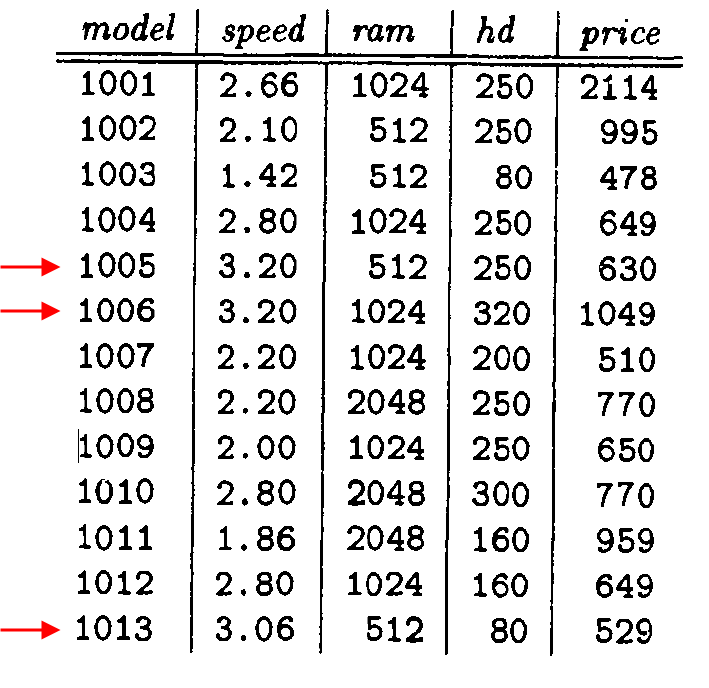
\includegraphics[width=0.4\linewidth]{images/worksheet_2_solution_2.png}
        \end{center}

        \bigskip

        \underline{\textbf{Notes:}}

        \bigskip

        \begin{itemize}
            \item Select
            \begin{itemize}
                \item Is indicated by $\sigma$
                \item \textbf{Syntax:} $\sigma_{\text{QUERY}} \text{SCHEMA\_NAME}$
                \item e.g $\sigma_{length \geq 100 \textbf{ AND } studioName=`Fox'} \text{(Movies)}$

                \bigskip

                \begin{center}
                
\includegraphics[width=\linewidth]{images/worksheet_2_solution_1.png}
                \end{center}
            \end{itemize}
        \end{itemize}

        \item

        \bigskip

        \underline{\textbf{Notes:}}

        \bigskip

        \begin{itemize}
            \item Project
            \begin{itemize}
                \item Picks certain columns
                \item Is indicated by $\pi$
                \item \textbf{Syntax:} $\pi_{A_1, A_2, \cdots, A_n}$(Rel)
            \end{itemize}
        \end{itemize}


    \end{enumerate}
\end{enumerate}

\end{document}